% !Mode:: "TeX:UTF-8"
% \textbf{计算专题------无取值说理、直接代入}

\begin{defproblem}{T16-A06-01}%
\begin{onlyproblem}%
小明准备完成题目:化简:$(\square x^2+6x+8)-(6x+5x^2+2)$.发现系数``$\square$''印刷不清楚.

(1)他把``$\square$''猜成3,请你化简:$(3x^2+6x+8)-(6x+5x^2+2)$;

(2)他妈妈说:``你猜错了,我看到该题标谁答案的结果是常数.''通过计算说明原题中``$\square$''是几?
\end{onlyproblem}%
\begin{onlysolution}%
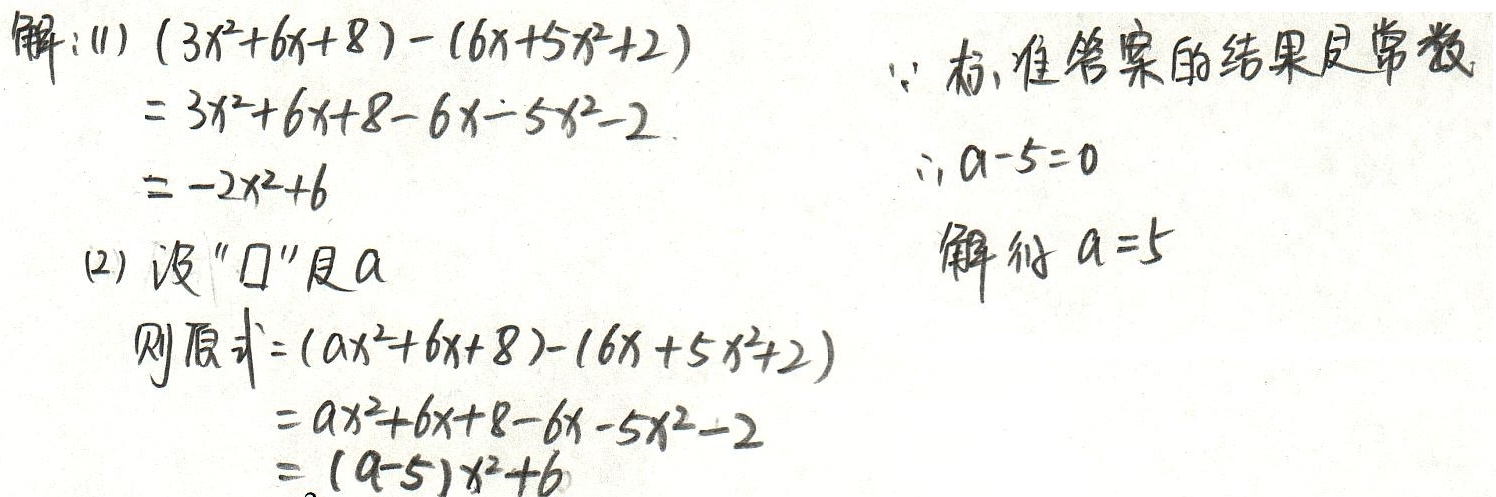
\includegraphics[width=8cm]{T16-A06-01.jpg}
\end{onlysolution}%
\end{defproblem}


\begin{defproblem}{T16-A06-02}%
\begin{onlyproblem}%
已知$T=\dfrac{a^2-9}{a(a+3)^2}+\dfrac{6}{a(a+3)}$.

(1)化简$T$;

(2)若正方形$ABCD$的边长为$a$,且它的面积为9,求$T$的值.
\end{onlyproblem}%
\begin{onlysolution}%
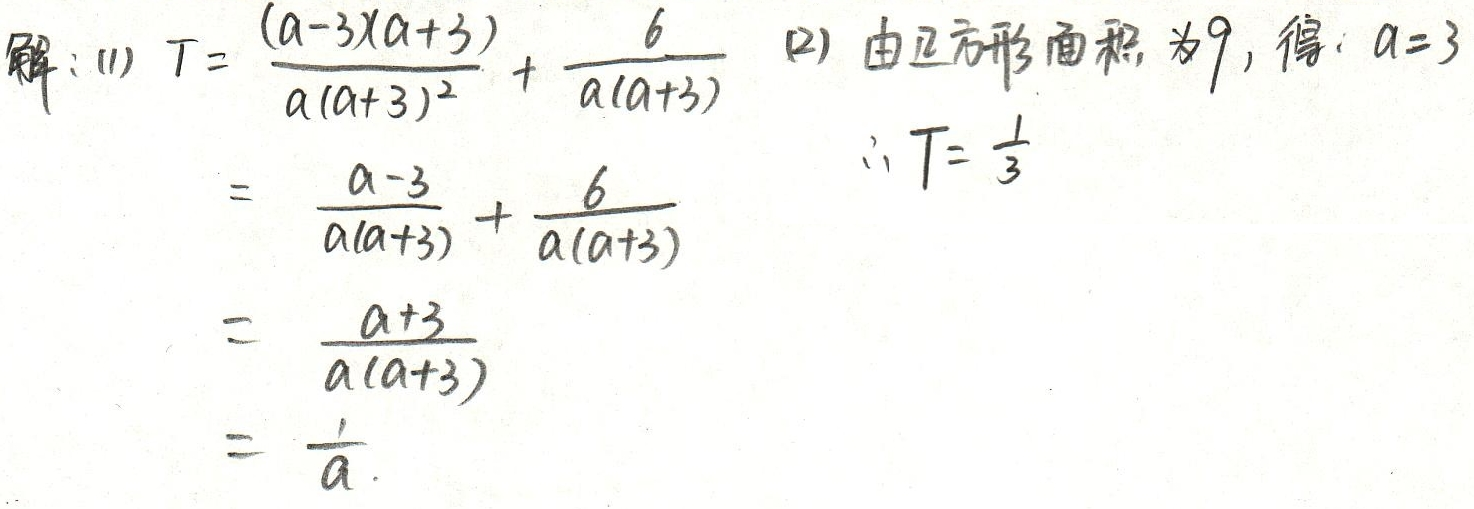
\includegraphics[width=\columnwidth]{T16-A06-02.jpg}
\end{onlysolution}%
\end{defproblem}


\begin{defproblem}{T16-A06-03}%
\begin{onlyproblem}%
阅读下列题目的解题过程:

已知$a$,$b$,$c$为$\triangle ABC$的三边,且满足$a^{2}c^{2}-b^{2}c^{2}=a^{4}-b^{4}$,试判断$\triangle ABC$的形状.

解:$a^{2}c^{2}-b^{2}c^{2}=a^{4}-b^{4}$(A)

$c^{2}(a^{2}-b^{2})=(a^{2}+b^{2})(a^{2}-b^{2})$(B)

$c^{2}=a^{2}+b^{2}$(C)

$\triangle ABC$是直角三角形

问:(1)上述解题过程,从哪一步开始出现错误?请写出该步的代号{\_}{\_}{\_}{\_};

(2)错误的原因为:{\_}{\_}{\_}{\_}{\_}{\_}{\_}{\_}{\_}{\_}{\_}{\_}{\_}{\_}{\_}{\_}{\_}{\_}{\_}{\_}{\_}{\_}{\_}{\_}{\_}{\_}{\_}{\_}{\_}{\_}{\_}{\_}{\_}{\_};

(3)本题正确的结论为:{\_}{\_}{\_}{\_}{\_}{\_}{\_}{\_}{\_}{\_}{\_}{\_}{\_}{\_}{\_}{\_}{\_}{\_}{\_}{\_}{\_}{\_}{\_}{\_}{\_}{\_}{\_}{\_}{\_}{\_}.
\end{onlyproblem}%
\begin{onlysolution}%
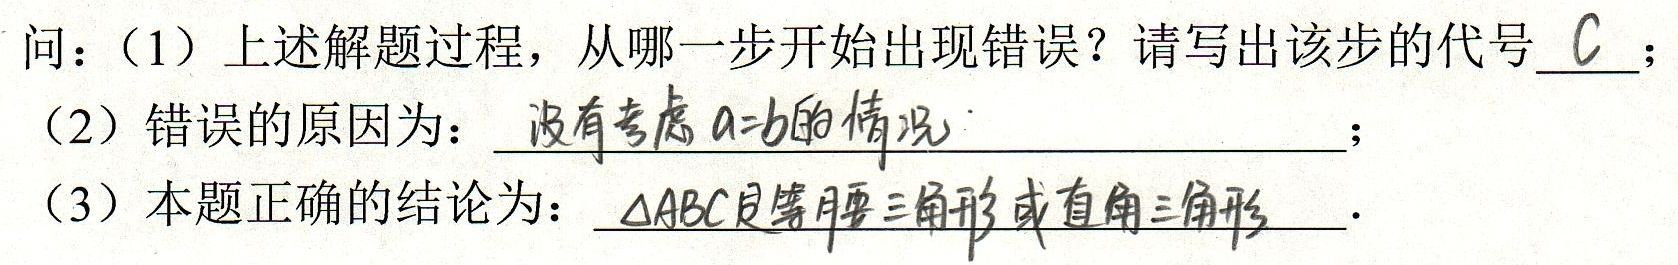
\includegraphics[width=\columnwidth]{T16-A06-03.jpg}
\end{onlysolution}%
\end{defproblem}


\begin{defproblem}{T16-A06-04}%
\begin{onlyproblem}%
已知关于$x$的方程$mx^{2}-3(m-1)x+2m-3=0$($m$为实数).

(1)求证:无论$m$为何值,该方程总有解.

(2)若方程有两个不相等的实数根,求$m$的取值范围.

(3)若$m$为整数,且方程的两个根均为正整数,求$m$的值.

(4)是否存在实数$m$,使方程的两个实数根互为相反数?如果存在,求出$m$的值;如果不存在,请说明理由.
\end{onlyproblem}%
\begin{onlysolution}%
(1)略;

(2)$m\ne 0$且$m\ne 3$;

(3)$m=-3$或$m=-1$或$m=3$;

(4)存在,$m=1$,理由略.
\end{onlysolution}%
\end{defproblem}


\begin{defproblem}{T16-A06-05}%
\begin{onlyproblem}%
先化简,再求值:$3x^2y-\left[2xy^2-4\left(\dfrac{1}{2}xy-\dfrac{3}{4}x^2y\right)+xy\right]+3xy^2$,其中$x=3$,$y=-1$.
\end{onlyproblem}%
\begin{onlysolution}%

\end{onlysolution}%
\end{defproblem}


\begin{defproblem}{T16-A06-06}%
\begin{onlyproblem}%
先化简,再求值:$3x^{2}y[6xy-2(4xy-3)+3x^{2}y]+1$,其中$x$和$y$满足$\vert2x+1\vert+(y-2)^{2}=0$.
\end{onlyproblem}%
\begin{onlysolution}%

\end{onlysolution}%
\end{defproblem}

